\documentclass[varwidth=17cm]{standalone}

\usepackage{tikz}
\usetikzlibrary{arrows}
\usepackage{pgfplots}
\pgfplotsset{compat=1.16}

% This file contains configuration shared between main file and figures

\usepackage{pifont}
\usepackage{xspace}
\DeclareUnicodeCharacter{2460}{\ding{172}\xspace}
\DeclareUnicodeCharacter{2461}{\ding{173}\xspace}

\usepackage{tikz}

\definecolor{HB9UFblue}{RGB}{0,61,165}
\definecolor{HB9UFred}{HTML}{ED135A}

\newcommand{\Ohm}{$\Omega$\xspace}


\newcommand{\uline}[1]{%
  \tikz[baseline=(todotted.base)]{
      \node[inner sep=1pt,outer sep=0pt] (todotted) {#1};
      \draw[color=HB9UFblue,thick] (todotted.south west) -- (todotted.south east);
  }%
}%
                           
\newcommand{\udash}[1]{%
  \tikz[baseline=(todotted.base)]{
      \node[inner sep=1pt,outer sep=0pt] (todotted) {#1};
      \draw[dashed,color=HB9UFred,thick] (todotted.south west) -- (todotted.south east);
  }%
}%


\begin{document}
    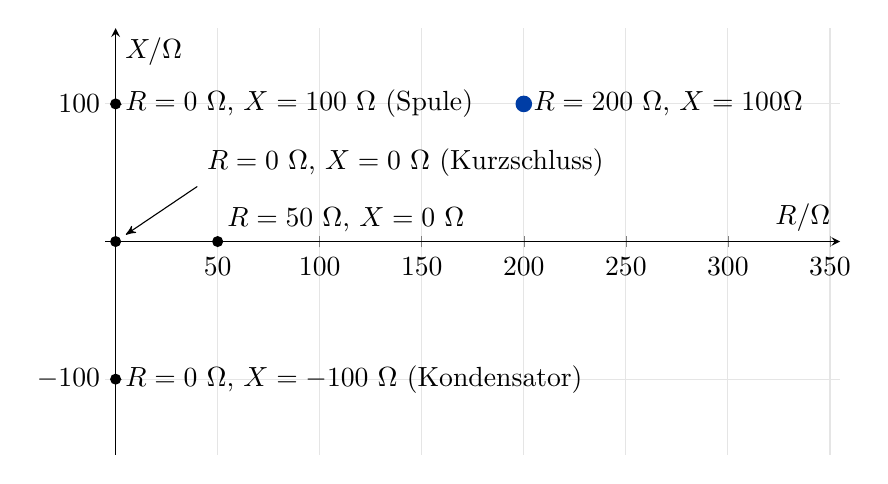
\begin{tikzpicture}
        \begin{axis}[
            xmin=-5, xmax=355,
            ymin=-155,ymax=155,
            xlabel={$R/\Omega$},
            ylabel={$X/\Omega$},
            grid=both,
            height=7cm,
            axis x line=center,
            axis y line=center,
            width=0.9\textwidth,
            major grid style={black!10}
        ]
        \fill [fill=HB9UFblue] (axis cs:200,100) circle [radius=3pt] node[right] {$R=200$~\Ohm, $X=100$\Ohm};
        \fill [fill=black] (axis cs:50,0) circle [radius=2pt] node[above right] {$R=50$~\Ohm, $X=0$~\Ohm};
        \fill [fill=black] (axis cs:0,100) circle [radius=2pt] node[right] {$R=0$~\Ohm, $X=100$~\Ohm (Spule)};
        \fill [fill=black] (axis cs:0,-100) circle [radius=2pt] node[right] {$R=0$~\Ohm, $X=-100$~\Ohm (Kondensator)};
        \fill [fill=black] (axis cs:0,0) circle [radius=2pt];
        \draw[stealth'-] (axis cs:5,5) -- (axis cs:40,40) node[above right] {$R=0$~\Ohm, $X=0$~\Ohm (Kurzschluss)};
    \end{axis}
    \end{tikzpicture}
\end{document}
